\label{sec:comparison}

In this chapter, we will compare Tamarin prover and Proverif under several points of view.
In particular, the comparison is going to cover the following topics:
\begin{itemize}
    \item Usability
    \item Expressiveness
    \item Efficiency
    \item Soundness and completeness
\end{itemize}

\section{Usability}
This may be the most complex property to evaluate as perceived usability can change with different levels of expertise and previous backgrounds. Of course, a user who has already used the \pic{} and Prolog would probably feel more comfortable with Proverif's formalisms. The usability of these tools for the formal verification of cryptographic protocols is, in general, difficult to establish. To the best of our knowledge, no study has been published regarding this specific topic. Another issue regards the formalization in Proverif, which was created by \MMNV{}, meaning we cannot know the problems that arose during modeling.

As we have seen, Tamarin offers a wide variety of built-in cryptographic primitives. While these are not hard to define, having predefined primitives allows for faster modeling compared to Proverif (where every single primitive must be defined).

The labeled multiset rewriting rules used by Tamarin is also more "low-level" than the applied \pic{}. As such, modeling using the latter is usually easier. A variant of the applied \pic{}, Sapic, has also been created to allow protocol specification in a stateful version of the applied \pic{} which is then automatically translated to labeled multiset rewriting rules and analyzed using Tamarin \cite{kremer:hal-00955869}. The authors' intentions were to create a sound and complete verification tool that was not ``error-prone and difficult'' as Tamarin, while keeping its features intact \cite{sapic-website}.

The security properties of both languages should be straightforward to model as these are based on well-known logical constructs. However, the guarded fragment of first-order logic used by Tamarin has a more complex syntax, which can probably intimidate beginners at first.

Assuming no previous knowledge, we can conclude that Tamarin's formalism and language might be slightly more complex than Proverif's.

\section{Expressiveness}
The various built-in theories offered by Tamarin are also very expressive. As we have seen in \cref{sub:built-in-equational-theories}, the \DiHe{}, the xor, and the bilinear-pairing equational theories are modeled faithfully. Moreover, Tamarin is one of the few tools able to model exclusive or \cite{xor_tamarin}.

\lstset{language=proverif}
The labeled multiset rewriting rules used by Tamarin is a more low-level formalism than then applied \pic{}. Nonetheless, rewriting rules allow encoding stateful protocols, which are not supported by the \Horncs{} used by Proverif. Moreover, as reported by S. Kremer and K. Robert \cite{kremer:hal-00955869}, many other efficient tools, such as AVISPA \cite{10.1007/11513988_27} or Maude-NPA \cite{Escobar2009}, fail to analyze protocols that require a non-monotonic global state (that is, some type of memory that can be read and altered). Proverif only supports the \lstinline{table} construct to save some information, but this construct does not support removal.

\section{Efficiency}
\begin{figure}
    \centering
    \subfloat[\Wct{} (ms)]{\label{a}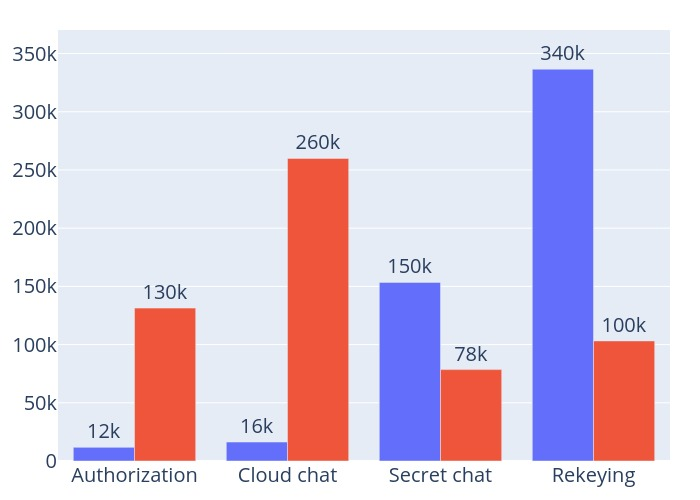
\includegraphics[width=.5\linewidth]{barplot_time}}\hfill
    \subfloat[\Mrss{} (kB)]{\label{b}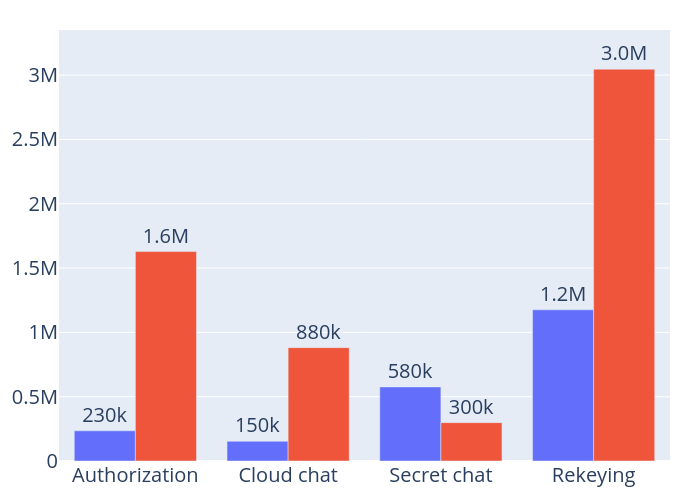
\includegraphics[width=.5\linewidth]{barplot_peak_size}}
    % \subfloat[CPU usage]{\label{c}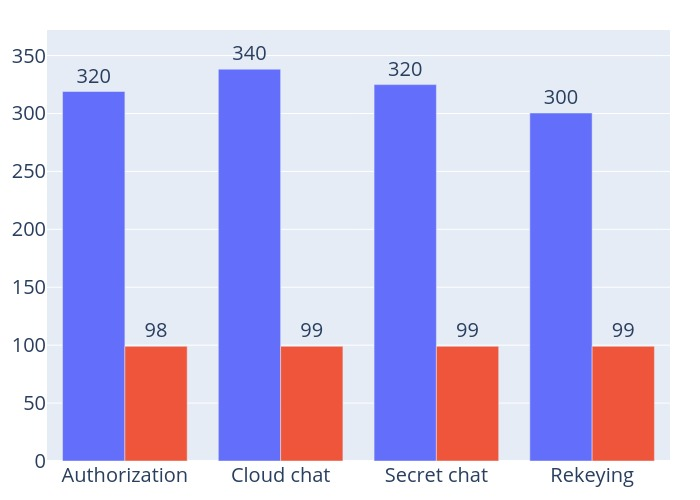
\includegraphics[width=.5\linewidth]{barplot_cpu_time}}
    \caption{In blue Tamarin, in red Proverif.\\\Wct{} and \mrss{} for every protocol and schema.}
    \label{fig:efficiency}
\end{figure}
In this section, we will compare the efficiency of Tamarin's and Proverif's MTProto2.0 formalization. Of course, the measured efficiency is indicative of this implementation only: as a small change can lead to both great performances or non-termination, this is only to be intended as the obtained efficiency of the current version of both implementations.

We consider two different metrics: \textit{\mrss{}} (in kB) and \textit{\wct{}} (in ms).

For the methodology, we followed the same approach of P. Lafourcade and M. Puys \cite{lafourcade:hal-01306395}. Benchmarks were run on an Intel(R) Core(TM) i5-7200U CPU @ 2.50GHz CPU with 16 GB or RAM. To get these three metrics we used the \lstinline{time} command (GNU version) \cite{time_command}. This version of time uses the \lstinline{getrusage} system call, which returns resource usage measures for a process, including our metrics. For each tool and protocol, we executed the proof 40 times. The entire process takes about 12 hours, depending on the hardware. For benchmarks, we used Proverif 2.02pl1 and Tamarin prover 1.6.0. Plots in \cref{fig:efficiency} show the mean value of each execution, while \cref{tab:efficiency} shows many relevant statistics. As we can see, the \mrss{} is usually significantly lower for Tamarin, while the \wct{} differs from protocol to protocol.

\begin{table}[!ht]
    \setlength\arrayrulewidth{1pt}
    \rowcolors{2}{gray!25}{white}
    \makebox[\textwidth][c]{
        \scalebox{0.9}{
            \begin{tabular}{c|cc|cc|c}
                \cline{2-5}
                \multicolumn{1}{l|}{}          & \multicolumn{2}{c|}{\textbf{Peak memory size (kb)}} & \multicolumn{2}{c|}{\textbf{Time (ms)}}                                                                                                                                 \\ \cline{2-6}
                \multicolumn{1}{l|}{}          & Tamarin                                             & Proverif                                & Tamarin   & Proverif  &                                                                                                       \\ \hline
                \multicolumn{1}{c|}{Mean}      & 234707.60                                           & 1628285.70                              & 11726.00  & 131329.50 & \multicolumn{1}{l}{}                                                                                  \\ \cline{1-6}
                \multicolumn{1}{c|}{Deviation} & 4965.62                                             & 149.06                                  & 381.48    & 198.86    & \multicolumn{1}{l}{}                                                                                  \\ \cline{1-6}
                \multicolumn{1}{c|}{Median}    & 234696                                              & 1628286                                 & 11740     & 131270    & \multicolumn{1}{l}{}                                                                                  \\ \cline{1-6}
                \multicolumn{1}{c|}{Min}       & 226000                                              & 1627968                                 & 10880     & 131140    & \multicolumn{1}{l}{}                                                                                  \\ \cline{1-6}
                \multicolumn{1}{c|}{Max}       & 245500                                              & 1628620                                 & 12330     & 131990    & \multicolumn{1}{l}{\parbox[t]{1em}{\multirow{-5}{*}{\rotatebox[origin=c]{90}{\textbf{Auth}}}}}        \\ \hline

                \multicolumn{1}{c|}{Mean}      & 153411.70                                           & 881417.40                               & 16290.50  & 259920.50 & \multicolumn{1}{l}{}                                                                                  \\ \cline{1-6}
                \multicolumn{1}{c|}{Deviation} & 4133.22                                             & 123.44                                  & 238.54    & 469.46    & \multicolumn{1}{l}{}                                                                                  \\ \cline{1-6}
                \multicolumn{1}{c|}{Median}    & 152588                                              & 881388                                  & 16280     & 260015    & \multicolumn{1}{l}{}                                                                                  \\ \cline{1-6}
                \multicolumn{1}{c|}{Min}       & 146384                                              & 881244                                  & 15760     & 259040    & \multicolumn{1}{l}{}                                                                                  \\ \cline{1-6}
                \multicolumn{1}{c|}{Max}       & 163840                                              & 881628                                  & 16960     & 261000    & \multicolumn{1}{l}{\parbox[t]{1em}{\multirow{-5}{*}{\rotatebox[origin=c]{90}{\textbf{Cloud chat}}}}}  \\ \hline

                \multicolumn{1}{c|}{Mean}      & 576006.80                                           & 298242.10                               & 153397.75 & 78498.50  & \multicolumn{1}{l}{}                                                                                  \\ \cline{1-6}
                \multicolumn{1}{c|}{Deviation} & 20908.28                                            & 118.18                                  & 674.64    & 170.40    & \multicolumn{1}{l}{}                                                                                  \\ \cline{1-6}
                \multicolumn{1}{c|}{Median}    & 576940                                              & 298234                                  & 153465    & 78500     & \multicolumn{1}{l}{}                                                                                  \\ \cline{1-6}
                \multicolumn{1}{c|}{Min}       & 529172                                              & 298032                                  & 151200    & 78220     & \multicolumn{1}{l}{}                                                                                  \\ \cline{1-6}
                \multicolumn{1}{c|}{Max}       & 618464                                              & 298488                                  & 154770    & 78940     & \multicolumn{1}{l}{\parbox[t]{1em}{\multirow{-5}{*}{\rotatebox[origin=c]{90}{\textbf{Secret chat}}}}} \\ \hline

                \multicolumn{1}{c|}{Mean}      & 1175407.70                                          & 3046324.80                              & 336571.25 & 103154.25 & \multicolumn{1}{l}{}                                                                                  \\ \cline{1-6}
                \multicolumn{1}{c|}{Deviation} & 14630.59                                            & 206.79                                  & 820.91    & 73.00     & \multicolumn{1}{l}{}                                                                                  \\ \cline{1-6}
                \multicolumn{1}{c|}{Median}    & 1175464                                             & 3046334                                 & 336415    & 103140    & \multicolumn{1}{l}{}                                                                                  \\ \cline{1-6}
                \multicolumn{1}{c|}{Min}       & 1138496                                             & 3045988                                 & 334970    & 103050    & \multicolumn{1}{l}{}                                                                                  \\ \cline{1-6}
                \multicolumn{1}{c|}{Max}       & 1212192                                             & 3046780                                 & 338460    & 103440    & \multicolumn{1}{l}{\parbox[t]{1em}{\multirow{-5}{*}{\rotatebox[origin=c]{90}{\textbf{Rekeying}}}}}    \\
            \end{tabular}
        }
    }
    \caption{Efficiency of the two models for every protocol.}
    \label{tab:efficiency}
\end{table}


\section{Soundness and completeness}
Let us define what soundness and completeness of formal verification tools mean. Definitions are the same given by M. Furer et al. \cite{furer1989completeness}.
\textbf{Soundness} means that any statement that can be proven is valid. A proof system is sound if whenever we can prove something, it is also true. As a formula:

\begin{equation}
    \Gamma \vdash Q \quad \Longrightarrow \quad \Gamma \models Q
\end{equation}

\textbf{Completeness} means that the proof system is powerful enough to prove any valid statement (in some class). In other words, a proof system is complete if whenever something is true, it can be proved to be so. As a formula:

\begin{equation}
    \Gamma \models Q \quad \Longrightarrow \quad \Gamma \vdash Q
\end{equation}

As we can see, soundness is a critical property. Unsound proof systems allow proofs of false statements. In the case of cryptographic protocol verification, this may imply, in the best-case scenario, that the prover yields a proof for a false attack. In the worst case, the tool may miss an attack, which is far more problematic.
Completeness, on the contrary, is a nice-to-have property. Incompleteness means there are some true properties for which there are no proofs in our formal system. \cite{slides_on_sound_complete}.

The foundational papers of Proverif and Tamarin prover respectively assert that:
\begin{itemize}
    \item Proverif is sound, but not complete \cite{ProverifManual};
    \item Tamarin is both sound and complete \cite{TamarinFoundations, TamarinFoundationsExtended, xor_tamarin}.
\end{itemize}

